%%%%%% CMB-S4 Simulations and Data Analysis Chapter  %%%%%%%%%%%%%%%%
 
\chapter{Data Analysis, Simulations \& Forecasting}
%\renewcommand*\thesection{\arabic{section}}

%%%%%%%%%%%%%%%%%%%%%%%%%%%%%%%%%%%%%%%%%%%%%%%%%%%%%%%%%%%
%%%%%%%%%%%%%%%%%%%%%%%%%%%%%%%%%%%%%%%%%%%%%%%%%%%%%%%%%%%
%%%%%%%%%%%%%%%%%%%%%%%%%%%%%%%%%%%%%%%%%%%%%%%%%%%%%%%%%%%
%%%%%%%%%%%%%%%%%%%%%%%%%%%%%%%%%%%%%%%%%%%%%%%%%%%%%%%%%%%

\begin{center}
{\it \small (send any feedback on this chapter to 
\href{mailto:s4_forecasting@cosmo.uchicago.edu}{s4\_forecasting@cosmo.uchicago.edu}
or
\href{mailto:s4_skymodel@cosmo.uchicago.edu}{s4\_skymodel@cosmo.uchicago.edu})}
\end{center}

\section{Introduction}

Extracting science from a CMB dataset is a complex, iterative process requiring expertise in both physical and computational sciences. In this chapter we start with an overview of the data analysis pipeline before diving more deeply into its subsets - time-ordered data processing, map-domain processing, and the estimation of statistics and parameters. We then discuss the drivers for the simulation pipeline, and describe in detail its sky modeling and data simulation subsets. From these pieces we then assemble the full production simulation and data analysis pipeline, including its various feedback loops, and consider the computational challenges posed by its implementation and execution. Finally we detail some approaches to mission forecasting, bypassing the most computationally challenging steps in the production pipeline in order to be able to explore the full instument and observation parameter space. Throughout our goal is to describe the current state of the art, note the particular challenges posed by \cmbexp\, and describe how these challenges might be addressed.

\section{Data Analysis Overview}

The central challenge of CMB data analysis is to reduce both the systematic and statistical uncertainties in the data to a sufficient level to enable well-constrained estimates of the parameters of cosmology and fundamental physics. Typically this is achieved through an iterative process, first mitigating the systematic effects exposed in the particular data domain, and then performing a data-compressing domain transformation in order to reduce the statistical uncertainty by increasing the signal-to-noise.

\begin{figure}[htbp]
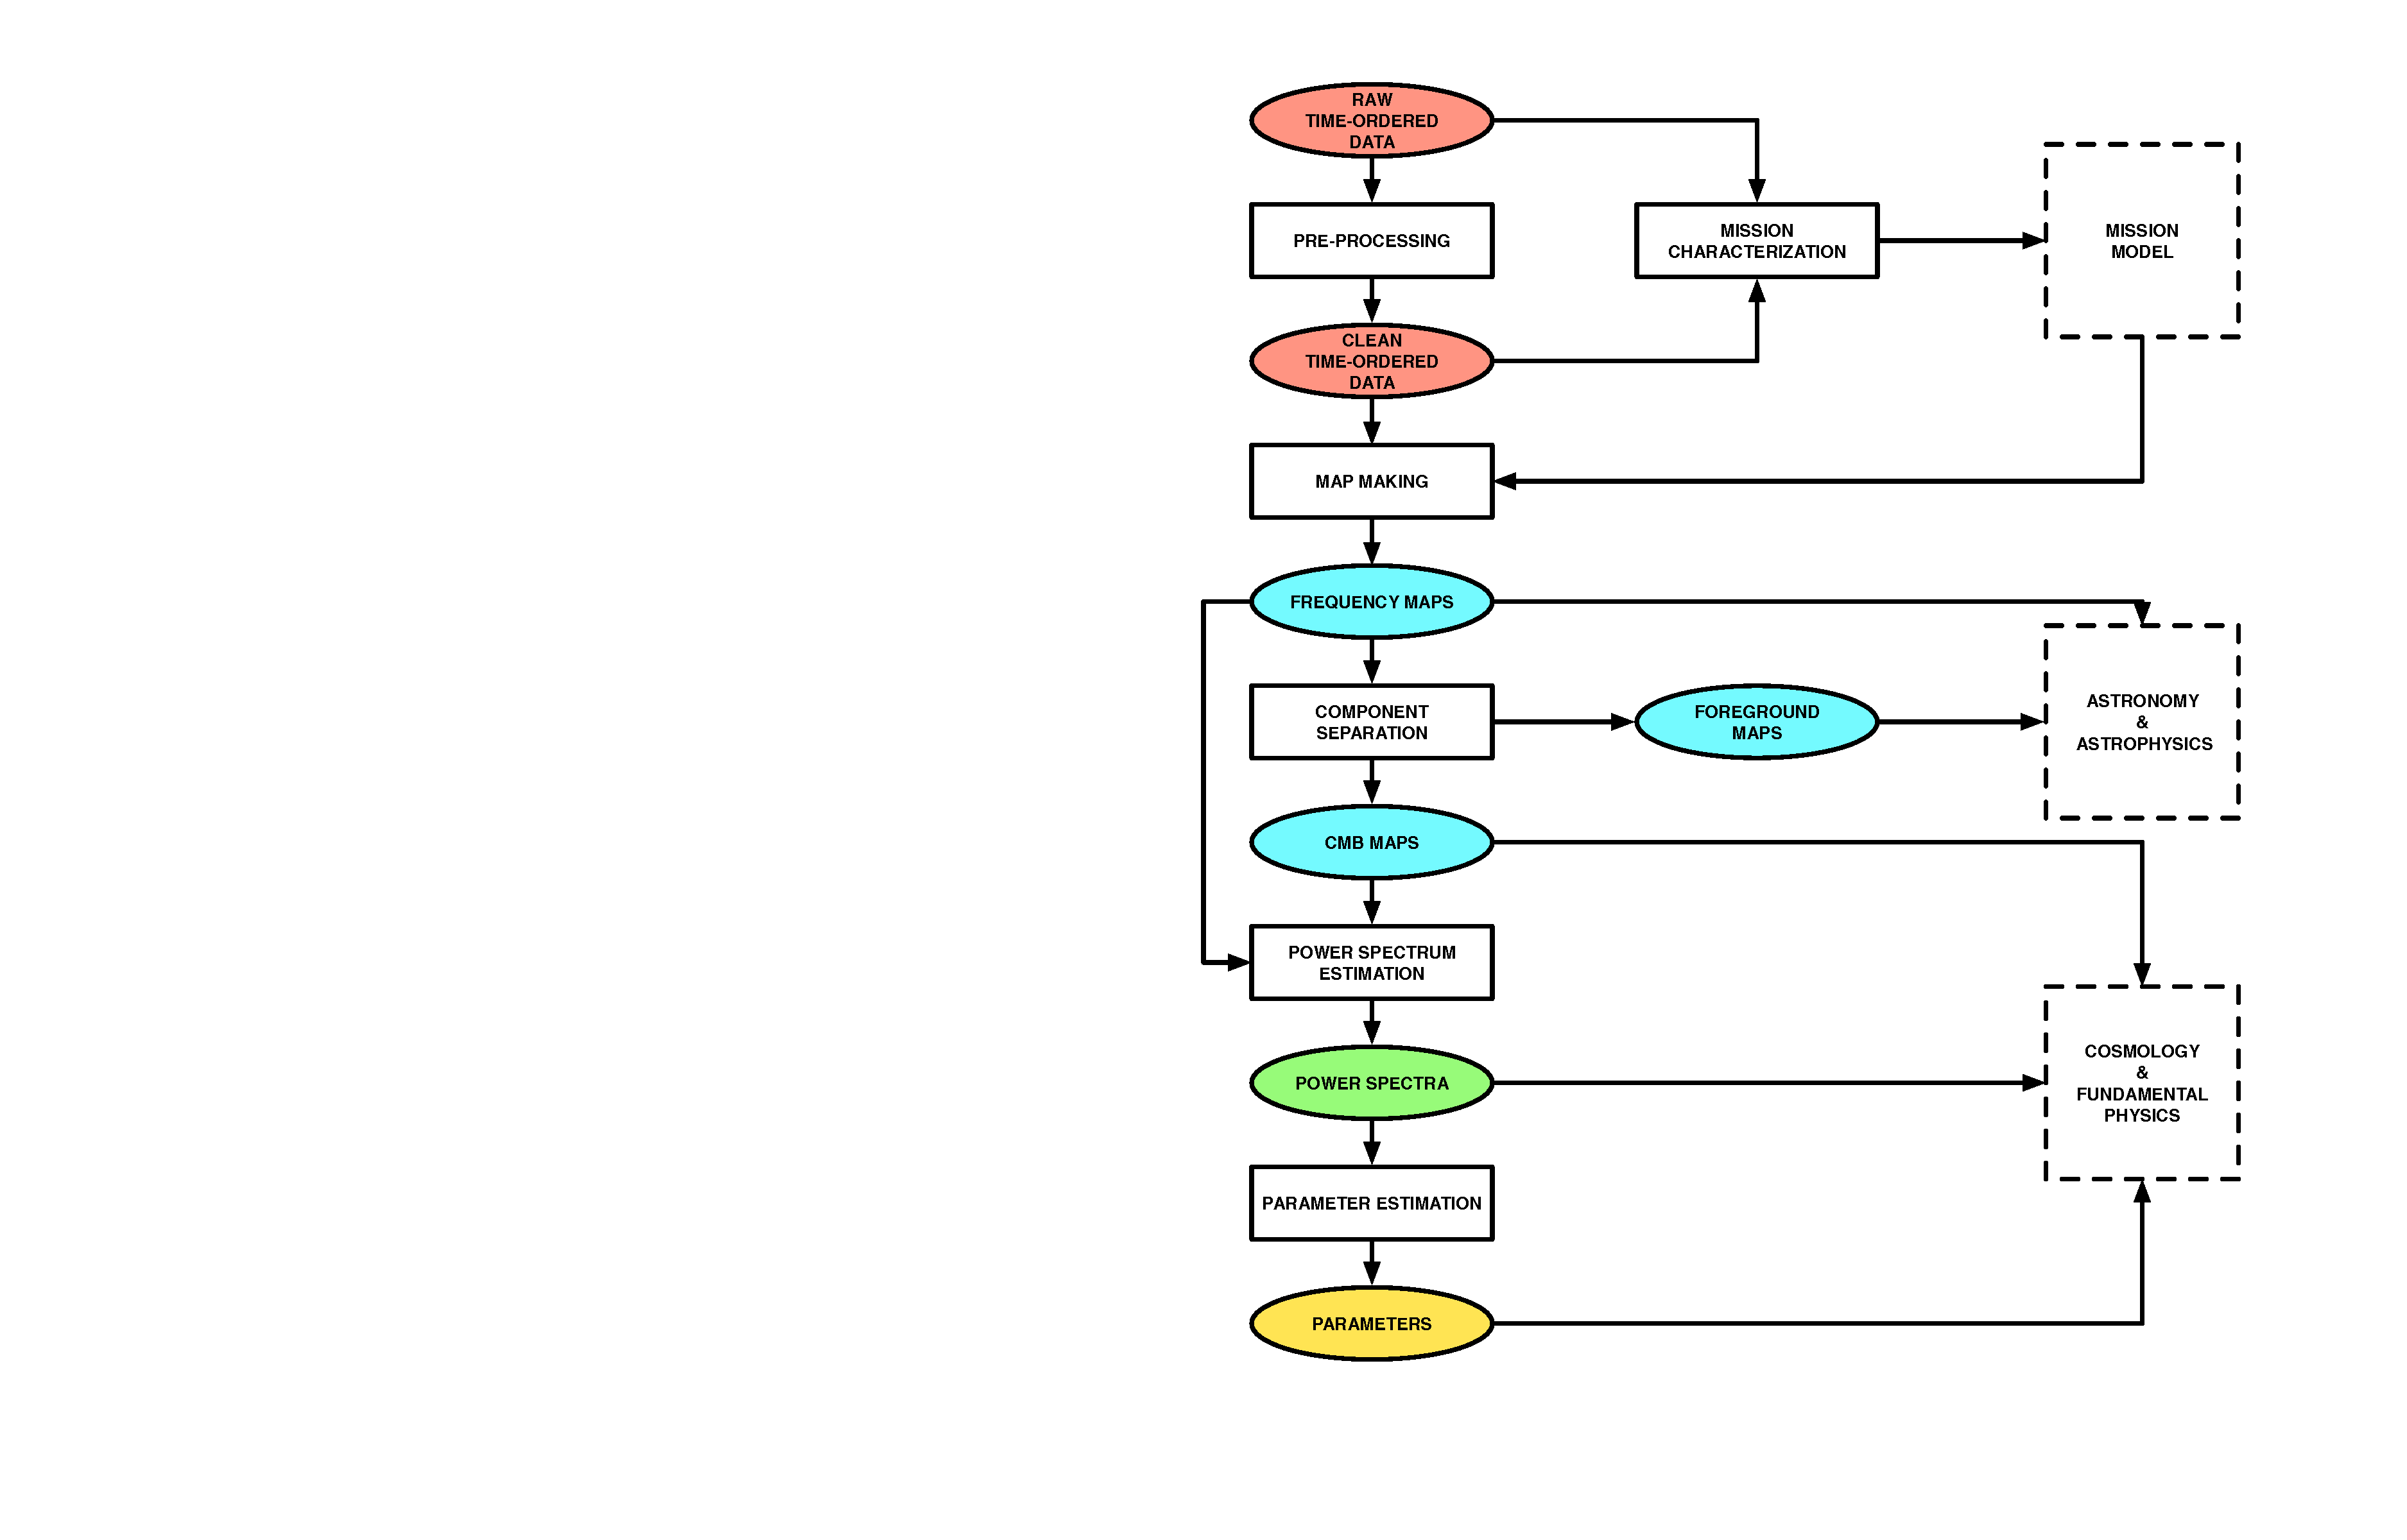
\includegraphics[width=0.7\textwidth]{Analysis/da}\\
\caption{The schematic CMB data analysis pipeline, showing the reduction from time-samples (red) to map-pixels (blue) to spectral-multipoles (green), including processes to reduce both systematic (horizontal) and statistical (vertical) uncertainties.}
\label{fig_da}
\end{figure}

As illustrated in Figure \ref{fig_da}, this analysis proceeds in a series of steps:
\begin{description}
\item[ Pre-processing:] The raw time-ordered detector data are calibrated, and gross time-domain systematics are either removed (typically by template subtraction, filtering, or marginalization) or flagged. The goal here is to make the real data match a model that will underpin all subsequent analyses.
\item[Map-making:] At each observing frequency, estimates of the intensity I and the Stokes Q- and U-polarizations of the sky signal are extracted from the cleaned time-ordered data based on their spatial stationarity, typically using some degree of knowledge of the instrument's noise properties.
\item[Foreground Cleaning:] If a sufficient number of frequency maps are available, the CMB can be separated from foreground emission based on its unique spectral signature; if insufficient frequency maps are available then we must use a combination of masking and marginalizing over foreground templates from other sources.
\item[Power spectrum estimation \& higher-order statistics:] The observed two-point correlation functions (power spectra) of the CMB temperature T and E- and B-mode polarizations are estimated from the CMB and/or frequency maps; various higher-order (typically three- and four-point) correlation functions may also estimated from the CMB maps.
\item[Post-processing]: The primordial power spectra are derived from the observed spectra, with the details of this step depending on both the input maps and the algorithms used in the spectral estimation; examples of this step include debiasing of pseudo-spectra, delensing, and spectral-domain point-source removal.
\item[Parameter estimation:] The best-fit parameters for any cosmological model are derived by comparing the theoretical correlation function(s) predicted by the model with the data.
\end{description}

Note however that the data can only remain a sufficient statistic at each step in the reduction if we also propagate its full covariance matrix. This is an ${\cal N}_b \times {\cal N}_b$ matrix in the dimension of the basis, so its construction, manipulation and reduction typically poses the greatest computational challenge to this analysis. In particular the full pixel-domain data covariance matrix is generally dense and unstructured, requiring O(${\cal N}_p^3$) operations to build and O(${\cal N}_p^2$) bytes to store. A mission that covers a fraction of the sky \fsky\ with a beam of $b$ arcminutes generates O($10^9 \, \fsky/b^2$) pixels per CMB component per observing frequency, so that increases in sky fraction, resolution, polarization sensitivity or frequency coverage (as have been the science drivers to date) necessarily increases ${\cal N}_p$. For the last decade or more the computational intractability of the resulting pixel-domain matrices has forced us to replace explicit covariance propagation with Monte Carlo methods in all but a limited set of small sky fraction/low resolution cases -- although it should be noted that, as outlined previously, this case may be of great interest for determining the tensor-to-scalar ratio $r$.

\input Analysis/tod_processing.tex

\input Analysis/component_separation.tex

\input Analysis/statistics_parameters.tex

\section{Simulation Overview}
Simulations of a CMB mission's data play a number of critical roles; specifically they are required for
\begin{itemize}
\item Mission design and development: ensuring that the mission is capable of meeting its science goals.
\item Validation and verification: ensuring that all of our data analysis tools meet their requirements and specifications.
\item Uncertainty quantification and debiasing: providing an alternative to the full data covariance matrix when this is computationally intractable.
\end{itemize}

As shown in Figure \ref{fig_sim}, given a mission model (both instrument and observation) and a sky model (both CMB and extra-galactic and galactic foregrounds) we can generate a simulation of the mission data in any of its domains. However, there is an inevitable trade-off between how representative the simulation is of real data and the complexity of the input models and computational cost of generating the simulation. The choice of the simulation data domain will then be determined by the balance between the realism requirements and the complexity/cost constraints for the particular task at hand.

\begin{figure}[htbp]
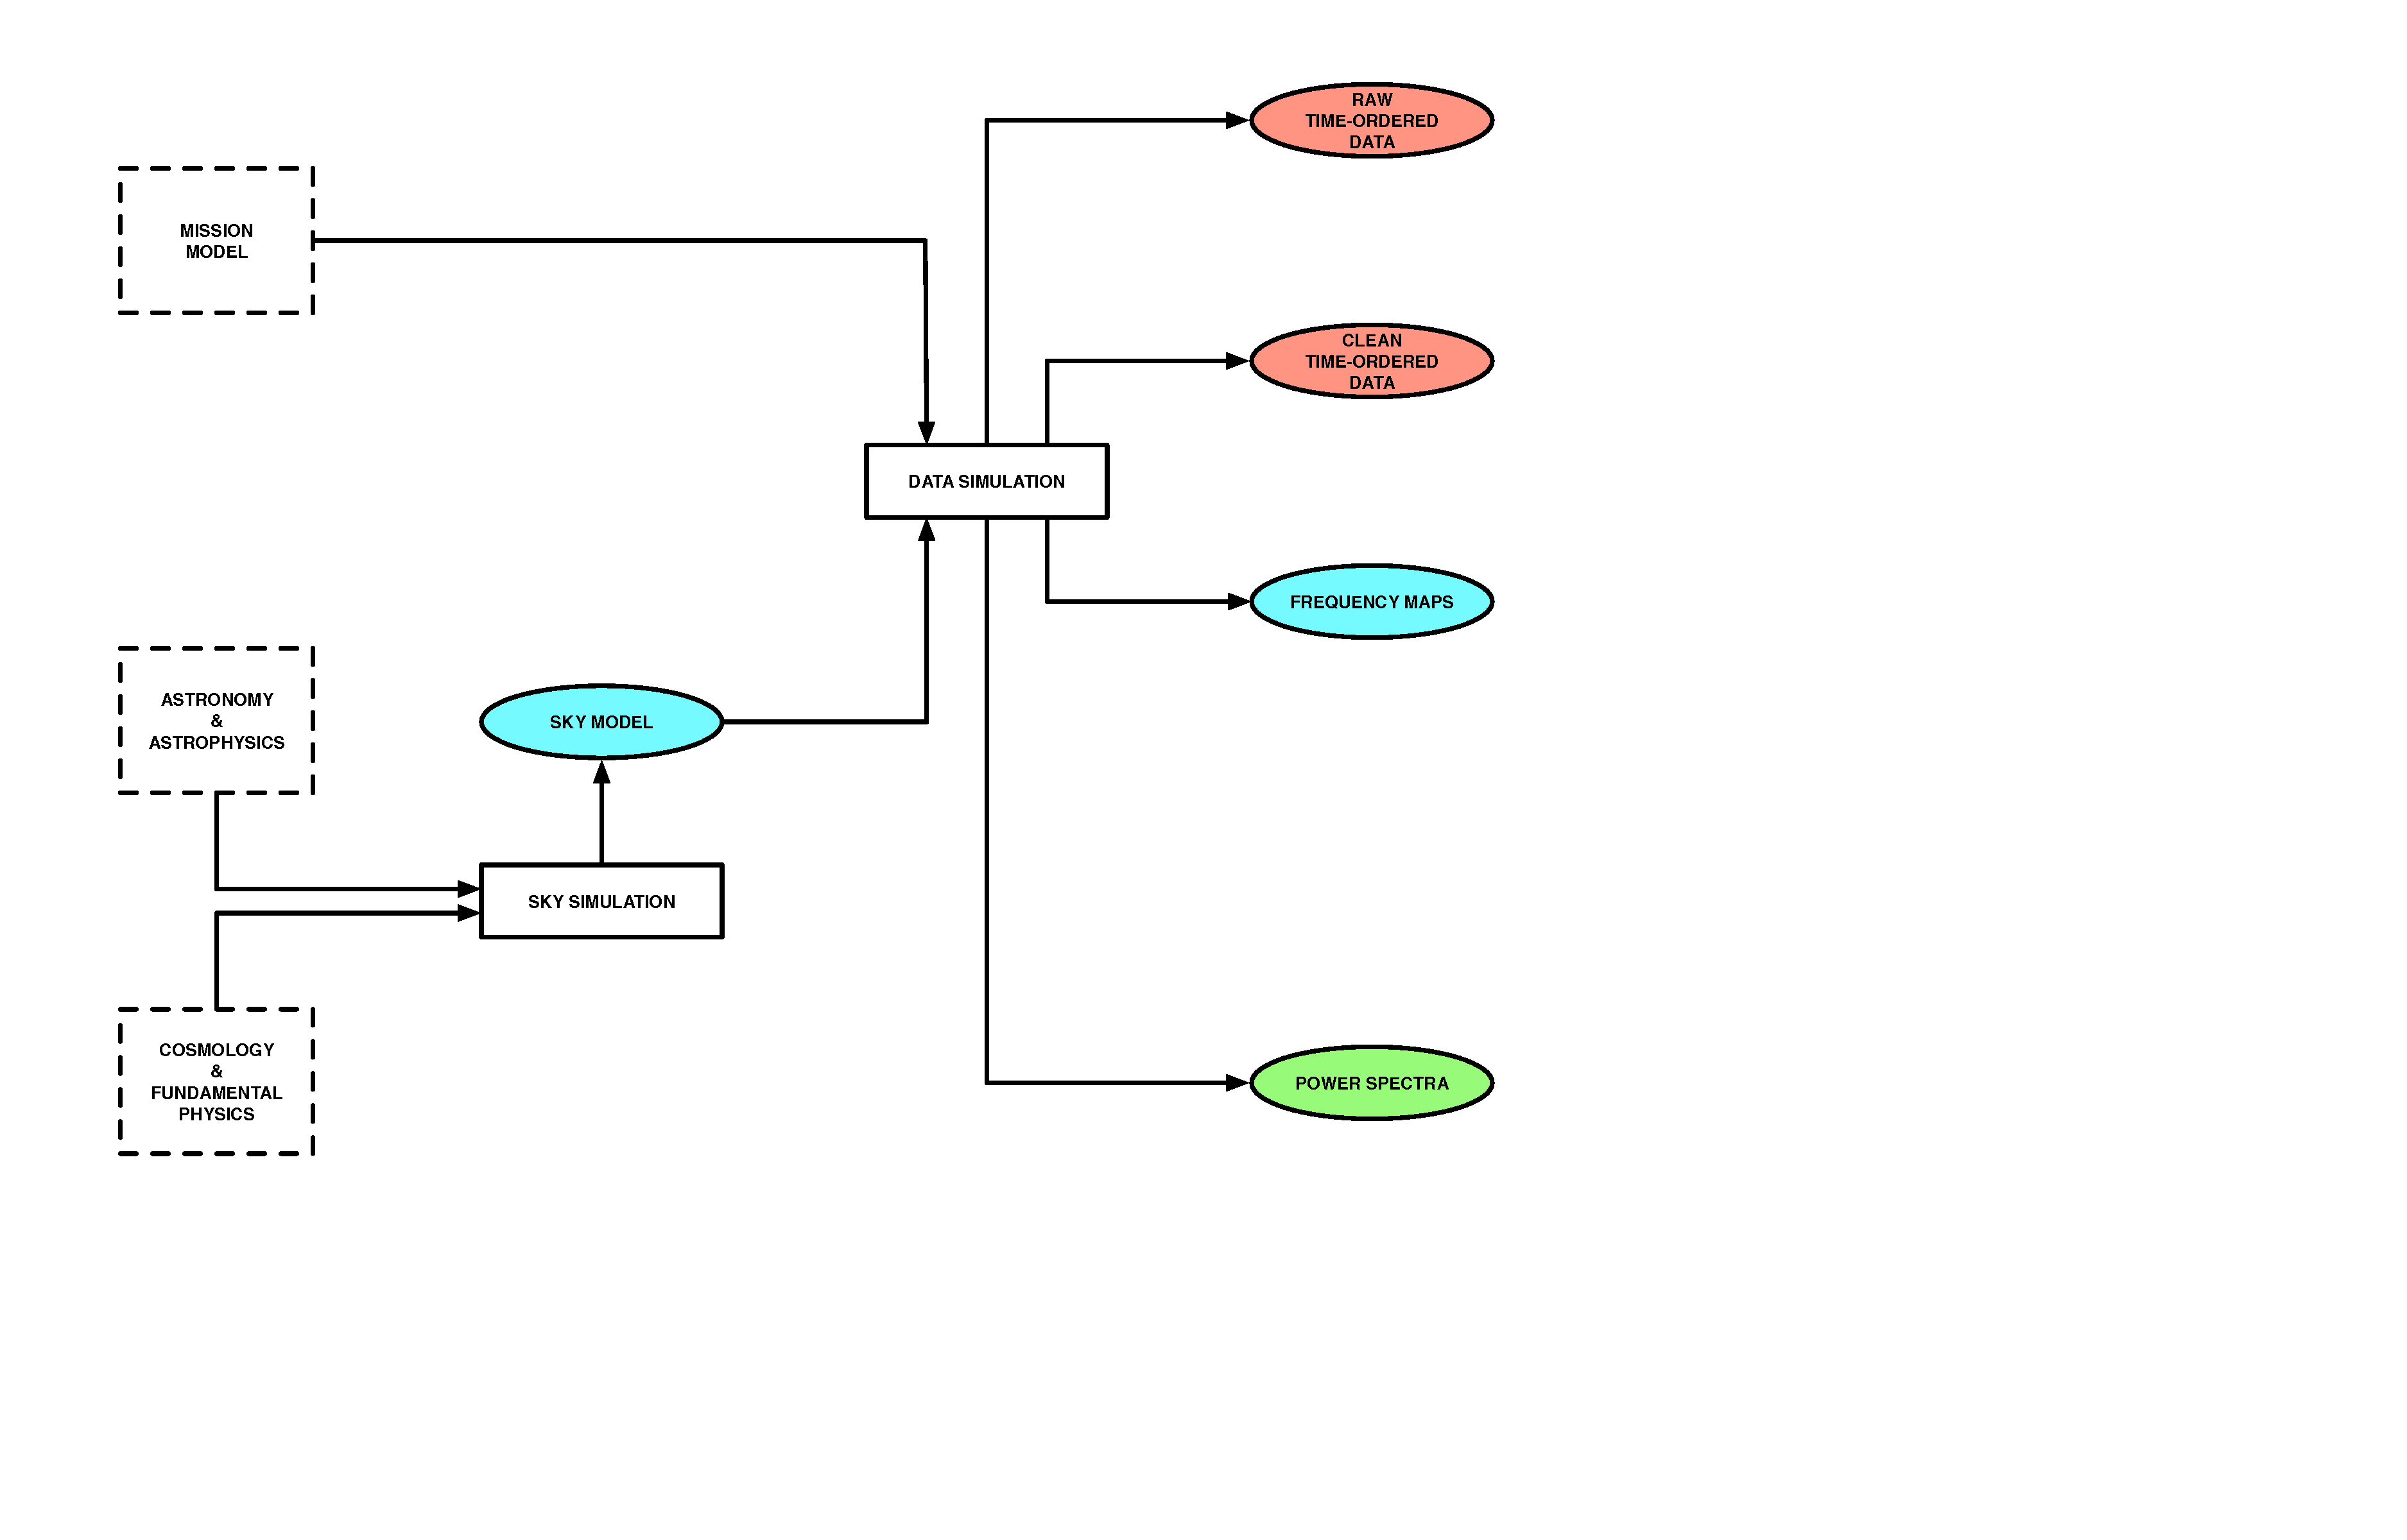
\includegraphics[width=0.6\textwidth]{Analysis/sim}\\
\caption{The CMB simulation pipeline, including both mission-independent sky modeling and mission-specific data simulation in the time (red), pixel (blue) and spectral (green) domains.}
\label{fig_sim}
\end{figure}

The generation of the input mission and sky models are themselves far from trivial tasks. The mission model is typically derived from pre-deployment measurements of the instrument properties refined by characterization from the data themselves, together with ancilliary telescope and environmental data characterizing the observation; the sky model requires its own dedicated simulation capability which - since it is independent of the details of any single mission - can be a community-wide endeavor.

\input Analysis/sky_modeling.tex

\input Analysis/data_simulation.tex

\input Analysis/production.tex

\input Analysis/forecasting.tex

%\bibliography{cmbs4}

%%
%% Populate the .bib file with entries from SPIRES Bibtex (preferred)
%% or ADS Bibtex (if no SPIRES entry).
%%  SPIRES will also supply the CITATION line information; please include it.
%%


